\documentclass[conference,harvard,brazil,english]{sbatex}
\usepackage[T1]{fontenc}
\usepackage{textcomp}
\usepackage[utf8]{inputenc}
\usepackage{graphicx}
\usepackage{url}
\usepackage{bbding}
\usepackage{fixltx2e}

\graphicspath{ {images/} }

\begin{document}
	\title{Obtendo mapa de profundidade de imagens estéreo}
	\author{Manoel Vieira Coelho Neto}{vieiranetoc@gmail.com}
	\address{SQS 203 Bloco J\\ Brasília, DF, Brasil}
	
	\twocolumn[{
		\maketitle		
	}]
	\selectlanguage{Brazil}
	\section{Objetivos}
		\par Este relatório tem como objetivo extrair informação de distância entre os objetos da imagem e a câmera. Para isso foi necessário o uso da biblioteca OpenCV, linguagem C++ e alguns algoritmos explicitados ao longo do texto (como busca por SAD). Para que seja possível a obtenção do mapa, é necessário que as duas imagens estejam retificadas e sejam epipolares (linhas coincidentes), tais imagens são chamadas de imagens estéreo. A imagem resultante do processo é o mapa de profundidade, com ele podemos fazer reconstrução de ambientes em 3D, por exemplo.
	\section{Introdução}
		\par A visão humana consegue medir distâncias com precisão graças à livre movimentação dos olhos em direção a um ponto de foco, a distância entre os olhos e o ponto é dada por $ d = \frac{c}{2tg(\alpha/2)}$, onde $c$ é a distância entre os olhos e $\alpha$ o ângulo entre o ponto e os olhos.	
		\par Associado ao foco $f$, temos o ponto $P$ interno à câmera. Sabendo a diferença no eixo $x$ entre o ponto $P$ de cada um dos olhos(D,E) e o ponto $P\textsubscript{D}$ e $P\textsubscript{E}$ podemos calcular a distância entre a câmera e o ponto do mundo por meio da fórmula:\newline 
		\par $Z= \frac{bf}{(X\textsubscript{L} - X\textsubscript{R})}$
		\par {  \tiny  Essa formula pode ser obtida através de semelhança de triângulos, a imagem segue no final do texto como anexo}	
		\par Imagens estéreos são obtidas a partir de duas diferentes angulações da câmera em torno do objeto, tal qual os olhos humanos, ao fazer isso sem mudar o eixo y da câmera teremos imagens epipolares, ou seja, as linhas da imagem à esquerda são coincidentes com as linhas da imagem à direita. Assim, há um pixel em cada imagem na mesma linha associado à um mesmo ponto da imagem. Aqueles pontos que não tiverem coincidência entre si são, portanto, nosso \textit{background} e não pertencem ao(s) objeto(s) de interesse.
	
	\section{Metodologia}
		\par O algoritmo usado neste trabalho é conhecido como \textit{Window-based matching}, ou correspondência baseada em janela em tradução livre. E para qualquer algoritmo de profundidade estéreo é necessário a retificação das duas imagens de forma que possa se achar os pixeis correspondentes nas duas imagens.
		\par Para determinar os pixeis coincidentes nas imagens foi feito uso do algoritmo SAD, onde cria-se um \textit{template} de tamanho \textit{w} que será uma matriz quadrada a ser comparada com uma região de mesma ordem em torno do pixel da outra imagem, onde cada elemento da matriz de comparação resultante será a diferença absoluta entre os elementos (i,j), ao final, somamos todos os elementos da matriz de comparação e chamamos esse processo de SAD (\textit{sum of absolut differences}), aquele pixel com menor sad é dito o pixel correspondente na imagem à direita, iteramos cada pixel de uma linha da imagem da esquerda com todos os pixeis da mesma linha na imagem à direita e o processo se repete para todas as linhas das imagens.\textsuperscript{1}
		\par Calcula-se então a distância Z para cada pixel da imagem usando da fórmula de Z mostrada acima, para aqueles pontos em que 
		$(X\textsubscript{L} - X\textsubscript{R}) = 0$ associamos um número absurdamente grande ao pixel de Z, para indicar que há correspondência total naquele valor de (x,y) da imagem Z. Então nossa imagem normalizada entre 0 e 255 deve ser nosso mapa de profundidade.
	\section{Resultados} 
		\par Como resultado temos as imagens abaixo, as imagens originais foram upadas no site do imgur pois sua resolução é alta e não cabe nesse documento:\newline
		\par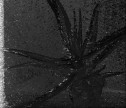
\includegraphics{image/gray}\newline
			
				\url{http://imgur.com/MzQWSYo} \newline
		\par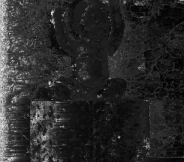
\includegraphics{image/baby.png}\newline
				\newline\url{http://imgur.com/3RuP5I7}\newline
			
		
			
		
	\section{Conclusão e Discussões}
		\par É visível a imprecisão do algoritmo e a quantidade de ruídos presentes na imagem, há outros algoritmos que fazem o mapa de forma otimizada como o \textit{Ground Truth} ou \textit{SGBM(Semi-Global Block-Matching)}\textsuperscript{[2]},que talvez tivessem trazido resultados mais satisfatórios, a quantidade de ruído presente na imagem deve-se ao fato que há uma probabilidade de que haja um outro ponto na imagem com o $"sad"$ menor e devido a isso o valor daquele pixel seja discrepante em relação aos pontos, métodos de morfologia aplicados sobre a imagem também não trouxeram bons resultados quanto à diminuição do ruído, assim como método de \textit{threshold} binário também não foi favorável ao resultado almejado. Mas, ainda com a alta taxa de ruído, o objeto é distinguível na imagem de profundidade e pode-se dizer que dentro de uma boa margem de aceitação o resultado esperado foi obtido.
	
	\bibliography{exemplo}
	\textsuperscript{1}\cite{SAD_Algorithm}
	
	\textsuperscript{2}\cite{stereopaper}
	\cite{docsocv}
	
\end{document}